\documentclass[journal,12pt,twocolumn]{IEEEtran}
 %
 \usepackage{setspace}
 \usepackage{gensymb}
 \usepackage{siunitx}
 \usepackage{tkz-euclide} 
 \usetkzobj{all}
 \usepackage{textcomp}
 \usepackage{standalone}
 \usetikzlibrary{calc}

 %\doublespacing
 \singlespacing

 %\usepackage{graphicx}
 %\graphicspath{ {/user/utkarsh/desktop} }
 %\usepackage{amssymb}
 %\usepackage{relsize}
 \usepackage[cmex10]{amsmath}
 %\usepackage{amsthm}
 %\interdisplaylinepenalty=2500
 %\savesymbol{iint}
 %\usepackage{txfonts}
 %\restoresymbol{TXF}{iint}
 %\usepackage{wasysym}
 \usepackage{amsthm}
 %\usepackage{iithtlc}
 \usepackage{mathrsfs}
 \usepackage{txfonts}
 \usepackage{stfloats}
 \usepackage{bm}
 \usepackage{cite}
 \usepackage{cases}
 \usepackage{subfig}
 %\usepackage{xtab}
 \usepackage{longtable}
 \usepackage{multirow}
 %\usepackage{algorithm}
 %\usepackage{algpseudocode}
 \usepackage{enumitem}
 \usepackage{mathtools}
 \usepackage{steinmetz}
 \usepackage{tikz}
 \usepackage{circuitikz}
 \usepackage{verbatim}
 \usepackage{tfrupee}
 \usepackage[breaklinks=true]{hyperref}
 %\usepackage{stmaryrd}
 \usepackage{tkz-euclide} % loads  TikZ and tkz-base
 %\usetkzobj{all}
 \usetikzlibrary{calc,math}
 \usepackage{listings}
     \usepackage{color}                                            %%
     \usepackage{array}                                            %%
     \usepackage{longtable}                                        %%
     \usepackage{calc}                                             %%
     \usepackage{multirow}                                         %%
     \usepackage{hhline}                                           %%
     \usepackage{ifthen}                                           %%
   %optionally (for landscape tables embedded in another document): %%
     \usepackage{lscape}     
 \usepackage{multicol}
 \usepackage{chngcntr}
 \usepackage{amsmath}
 \usepackage{cleveref}
 %\usepackage{enumerate}

 %\usepackage{wasysym}
 %\newcounter{MYtempeqncnt}
 \DeclareMathOperator*{\Res}{Res}
 %\renewcommand{\baselinestretch}{2}
 \renewcommand\thesection{\arabic{section}}
 \renewcommand\thesubsection{\thesection.\arabic{subsection}}
 \renewcommand\thesubsubsection{\thesubsection.\arabic{subsubsection}}

 \renewcommand\thesectiondis{\arabic{section}}
 \renewcommand\thesubsectiondis{\thesectiondis.\arabic{subsection}}
 \renewcommand\thesubsubsectiondis{\thesubsectiondis.\arabic{subsubsection}}

 % correct bad hyphenation here
 \hyphenation{op-tical net-works semi-conduc-tor}
 \def\inputGnumericTable{}                                 %%

 \lstset{
 %language=C,
 frame=single, 
 breaklines=true,
 columns=fullflexible
 }
 %\lstset{
 %language=tex,
 %frame=single, 
 %breaklines=true
 %}
 \usepackage{graphicx}
 \usepackage{pgfplots}

 \begin{document}
 %


 \newtheorem{theorem}{Theorem}[section]
 \newtheorem{problem}{Problem}
 \newtheorem{proposition}{Proposition}[section]
 \newtheorem{lemma}{Lemma}[section]
 \newtheorem{corollary}[theorem]{Corollary}
 \newtheorem{example}{Example}[section]
 \newtheorem{definition}[problem]{Definition}
 %\newtheorem{thm}{Theorem}[section] 
 %\newtheorem{defn}[thm]{Definition}
 %\newtheorem{algorithm}{Algorithm}[section]
 %\newtheorem{cor}{Corollary}
 \newcommand{\BEQA}{\begin{eqnarray}}
 \newcommand{\EEQA}{\end{eqnarray}}
 \newcommand{\define}{\stackrel{\triangle}{=}}
 \bibliographystyle{IEEEtran}
 %\bibliographystyle{ieeetr}
 \providecommand{\mbf}{\mathbf}
 \providecommand{\pr}[1]{\ensuremath{\Pr\left(#1\right)}}
 \providecommand{\qfunc}[1]{\ensuremath{Q\left(#1\right)}}
 \providecommand{\sbrak}[1]{\ensuremath{{}\left[#1\right]}}
 \providecommand{\lsbrak}[1]{\ensuremath{{}\left[#1\right.}}
 \providecommand{\rsbrak}[1]{\ensuremath{{}\left.#1\right]}}
 \providecommand{\brak}[1]{\ensuremath{\left(#1\right)}}
 \providecommand{\lbrak}[1]{\ensuremath{\left(#1\right.}}
 \providecommand{\rbrak}[1]{\ensuremath{\left.#1\right)}}
 \providecommand{\cbrak}[1]{\ensuremath{\left\{#1\right\}}}
 \providecommand{\lcbrak}[1]{\ensuremath{\left\{#1\right.}}
 \providecommand{\rcbrak}[1]{\ensuremath{\left.#1\right\}}}
 \theoremstyle{remark}
 \newtheorem{rem}{Remark}
 \newcommand{\sgn}{\mathop{\mathrm{sgn}}}
 \providecommand{\abs}[1]{\left\vert#1\right\vert}
 \providecommand{\res}[1]{\Res\displaylimits_{#1}} 
 \providecommand{\norm}[1]{\left\lVert#1\right\rVert}
 %\providecommand{\norm}[1]{\lVert#1\rVert}
 \providecommand{\mtx}[1]{\mathbf{#1}}
 \providecommand{\mean}[1]{E\left[ #1 \right]}
 \providecommand{\fourier}{\overset{\mathcal{F}}{ \rightleftharpoons}}
 %\providecommand{\hilbert}{\overset{\mathcal{H}}{ \rightleftharpoons}}
 \providecommand{\system}{\overset{\mathcal{H}}{ \longleftrightarrow}}
 	%\newcommand{\solution}[2]{\textbf{Solution:}{#1}}
 \newcommand{\solution}{\noindent \textbf{Solution: }}
 \newcommand{\cosec}{\,\text{cosec}\,}
 \providecommand{\dec}[2]{\ensuremath{\overset{#1}{\underset{#2}{\gtrless}}}}
 \newcommand{\myvec}[1]{\ensuremath{\begin{pmatrix}#1\end{pmatrix}}}
 \newcommand{\mydet}[1]{\ensuremath{\begin{vmatrix}#1\end{vmatrix}}}
 %\numberwithin{equation}{section}
 \numberwithin{equation}{subsection}
 %\numberwithin{problem}{section}
 %\numberwithin{definition}{section}
 \makeatletter
 \@addtoreset{figure}{problem}
 \makeatother
 \let\StandardTheFigure\thefigure
 \let\vec\mathbf
 %\renewcommand{\thefigure}{\theproblem.\arabic{figure}}
 \renewcommand{\thefigure}{\theproblem}
 %\setlist[enumerate,1]{before=\renewcommand\theequation{\theenumi.\arabic{equation}}
 %\counterwithin{equation}{enumi}
 %\renewcommand{\theequation}{\arabic{subsection}.\arabic{equation}}
 \def\putbox#1#2#3{\makebox[0in][l]{\makebox[#1][l]{}\raisebox{\baselineskip}[0in][0in]{\raisebox{#2}[0in][0in]{#3}}}}
      \def\rightbox#1{\makebox[0in][r]{#1}}
      \def\centbox#1{\makebox[0in]{#1}}
      \def\topbox#1{\raisebox{-\baselineskip}[0in][0in]{#1}}
      \def\midbox#1{\raisebox{-0.5\baselineskip}[0in][0in]{#1}}
 \vspace{3cm}
 \title{Assignment 4}
 \author{Utkarsh Shashikant Surwade}
 \maketitle
 \newpage
 %\tableofcontents
 \bigskip
 \renewcommand{\thefigure}{\theenumi}
 \renewcommand{\thetable}{\theenumi}
 \begin{abstract}
 This document solves a question based on triangle.
 \end{abstract}
 All the codes for the figure in this document can be found at
 \begin{lstlisting}
 https://github.com/utkarshsurwade/Matrix_Theory_EE5609/tree/master/Assignment4
 \end{lstlisting}
 \section{Problem}
 E and F are respectively the mid-points of equal sides AB and AC of $\triangle{ABC}$.Show that BF = CE.
 \section{Solution}
\renewcommand{\thefigure}{1}
\renewcommand{\thefigure}{1}
\begin{figure}[!h]
\centering
\resizebox{\columnwidth}{!}{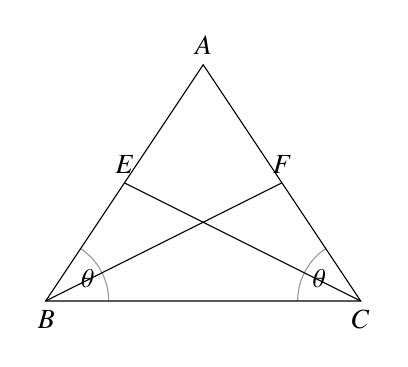
\begin{tikzpicture} 
        \coordinate (A) at (2, 3) {};
        \coordinate (B) at (0, 0) {};
        \coordinate (C) at (4, 0) {};
        \coordinate (E) at (1, 1.5) {};
        \coordinate (F) at (3, 1.5) {};
        \draw (A)node[above]{$A$}--(B)node[below]{$B$}--(C)node[below]{$C$}--cycle;
\draw (B)node[below]{}--(F)node[above]{$F$};
\draw (C)node[below]{}--(E)node[above]{$E$};
\tkzMarkAngle[fill= lightgray,size=0.8cm,%
opacity=.4](C,B,A)
\tkzLabelAngle[pos = 0.6](C,B,A){$\theta$}
\tkzMarkAngle[fill= lightgray,size=0.8cm,%
opacity=.4](A,C,B)
\tkzLabelAngle[pos = 0.6](A,C,B){$\theta$}
\end{tikzpicture}
}
\caption{Isosceles Triangle with mid-points E and F on equal sides}
\label{myfig}
\end{figure}
According to figure:
\begin{align}
\vec{(A-B)}+\vec{(B-F)} &= \vec{(A-F)}\\
\therefore \vec{(B-F)} &= \vec{(A-F)}-\vec{(A-B)}\\
\therefore \vec{(B-F)} &= \frac{1}{2}\vec{(A-C)}-\vec{(A-B)}
\end{align}
similarly,
\begin{align}
\vec{(A-C)}+\vec{(C-E)} &= \vec{(A-E)}\\
\therefore \vec{(C-E)} &= \vec{(A-E)}-\vec{(A-C)}\\
\therefore \vec{(C-E)} &= \frac{1}{2}\vec{(A-B)}-\vec{(A-C)}
\end{align}
Since AB = AC\\
$\therefore (AB)^2 = (AC)^2$\\
\begin{align}
\therefore\norm{\vec{(A-B)}}^2 = \norm{\vec{(A-C)}}^2
\end{align}
\begin{multline}
\norm{\vec{(A-B)}}^2+\frac{1}{4}\norm{\vec{(A-C)}}^2 -\vec{(A-C)}^T\vec{(A-B)} =\\
\norm{\vec{(A-C)}}^2+\frac{1}{4}\norm{\vec{(A-B)}}^2 -\vec{(A-B)}^T\vec{(A-C)} \end{multline}
\begin{multline}
(\frac{1}{2}\vec{(A-C)}-\vec{(A-B)})^T(\frac{1}{2}\vec{(A-C)}-\vec{(A-B)})=\\
(\frac{1}{2}\vec{(A-B)}-\vec{(A-C)})^T(\frac{1}{2}\vec{(A-B)}-\vec{(A-C)})
\end{multline}
\begin{align}
\norm{\vec{(B-F)}}^2 &= \norm{\vec{(C-E)}}^2\\
\therefore\norm{\vec{B-F}} &= \norm{\vec{C-E}}
\end{align}
Hence, BF is equal to CE
 \end{document}